\section{Resistência elétrica}

\frame{
	\frametitle{Resistência Elétrica}
	\begin{block}{Por que?}
		Quando aplicamos a mesma diferença de potencial às extremidades de barras de mesmas dimensões feitas de cobre e de vidro os resultados são muito diferentes.
		\begin{itemize}
			\item A característica do material que determina essa diferença é a \textbf{resistência elétrica}.
		\end{itemize}
	\end{block}
}

\frame{
	\frametitle{Resistência Elétrica}
	\begin{block}{Constante de proporcionalidade}
		Ao aplicar-se uma tensão $ U $, em um condutor qualquer se estabelece nele uma corrente elétrica de intensidade $ I $. Para a maior parte dos condutores estas duas grandezas são diretamente proporcionais, ou seja, conforme uma aumenta o mesmo ocorre à outra. \\
		$$ U \propto I $$
	\end{block}
}

\frame{
	\frametitle{Georg Simon Ohm}
	\centerline{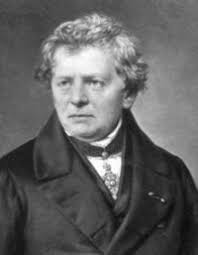
\includegraphics[width=0.3\linewidth]{Figuras/Ch12/ohm.png}}
	\begin{block}{Resistência Elétrica}
		\begin{itemize}
			\item Resistência elétrica pode ser caracterizada como a "dificuldade" encontrada para que haja passagem de corrente elétrica por um condutor submetido a uma determinada tensão
		\end{itemize}
	
		$$\text{unidade} = \text{ohm} \qquad [\si{\ohm}]$$
	\end{block}
}

\frame{
	\frametitle{Oposição à passagem de fluxo}
	\bigskip
	
	\centering
	
	\setmyunit{1.5cm}
	\begin{tikzpicture}
	\fill[blue] (0,0) -- ++(0,-3) -- ++(4,0) -- ++(0,0.5) -- ++(-1,0) -- ++(0,2.5) -- cycle;
	
	\draw (0,0) -- ++(0,-3) -- ++(4,0) ++(0,0.5) -- ++(-1,0) -- ++(0,2.5);
	
	\draw (0,0) -- +(0,0.5) (3,0) -- +(0,0.5);
	
	\draw[-Latex] (3,-2.75) ++(0,0.15) -- node[below=0pt] {Vazão} +(0.75,0);
	
	\draw[thick] (3.5,-2.5) -- ++(0,0.5) ++(0,0.4) circle (0.4);
	
	\foreach \x in {0,30,...,330}
	\draw (3.5,-1.6) ++(\x:0.35) -- +(\x:0.05);
	
	\draw (3.5,-1.6) -- +(25:0.4);
	
	\draw[decorate,decoration={brace,amplitude=10pt,mirror,raise=4pt}] (0,0) -- (0,-2.5) node[midway,left=15pt] {Altura};
	\end{tikzpicture}
%	\centerline{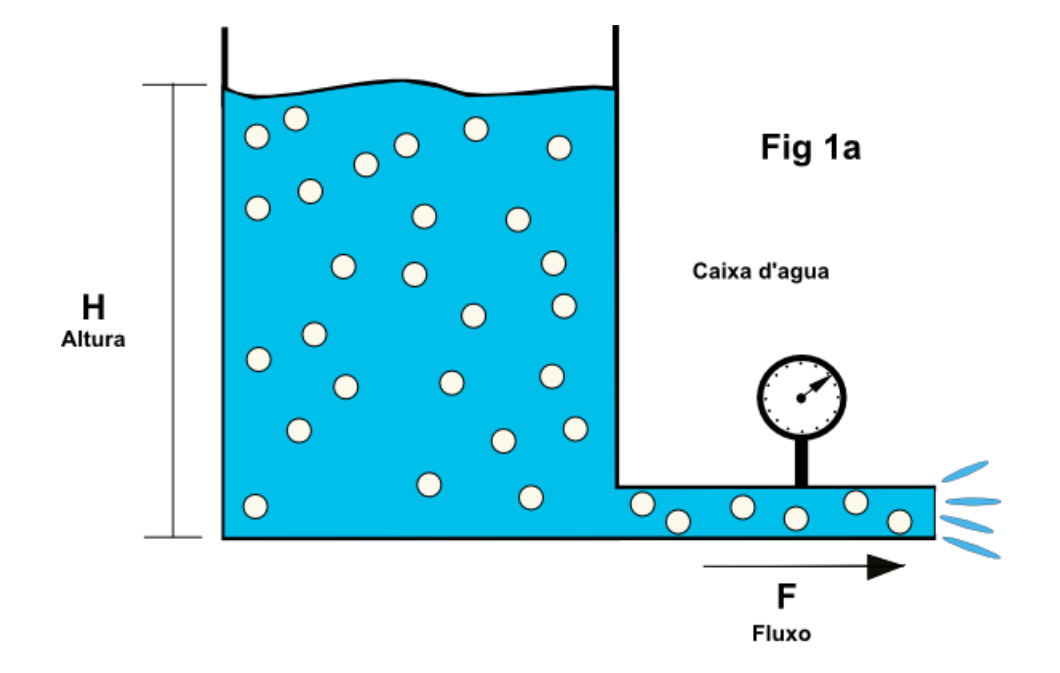
\includegraphics[width=0.9\linewidth]{Figuras/Ch12/ohm2.png}}
}

\frame{
	\frametitle{Condutância Elétrica}
	\begin{block}{Definição}
		É definida como a facilidade que uma corrente tem em passar por um condutor submetido à determinada tensão, ou seja, este é igual ao inverso da resistência
		
		$$G=\frac{1}{R} \qquad[\si{\ohm}^{-1}]$$
	\end{block}
}

\subsection{Resistores}
\frame{
	\frametitle{Resistores}
	\begin{block}{Definição}
		É um condutor cuja função em um circuito é introduzir uma certa resistência.
		
		\bigskip
		\centering
		\begin{circuitikz}[scale=1.25]
				\ctikzset{label/align=smart,bipoles/length=1.5cm}
				\draw (0,0) to[R,l_=\mbox{$R$},*-*] (2,0);
		\end{circuitikz}
	\end{block}

	\centerline{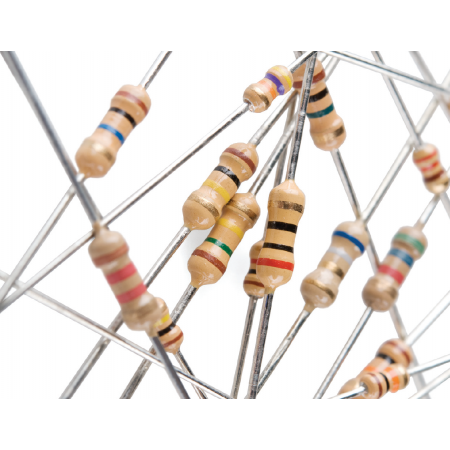
\includegraphics[width=0.3\linewidth]{Figuras/Ch12/resistores.png}}

}

\frame{
	\frametitle{Resistores}
	\begin{block}{}
		\begin{itemize}
			\item Se queremos usar água fria os resistores têm que trabalhar para limitar a sua intensidade de calor, ou seja, sua energia térmica.
		\end{itemize}
	\end{block}
	\centerline{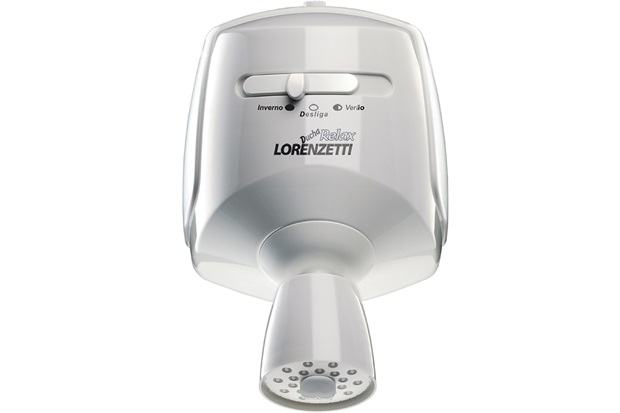
\includegraphics[width=0.8\linewidth]{Figuras/Ch12/chuveiro.png}}
	
}

\frame{
	\frametitle{Resistores ôhmicos e não ôhmicos}
%	\centerline{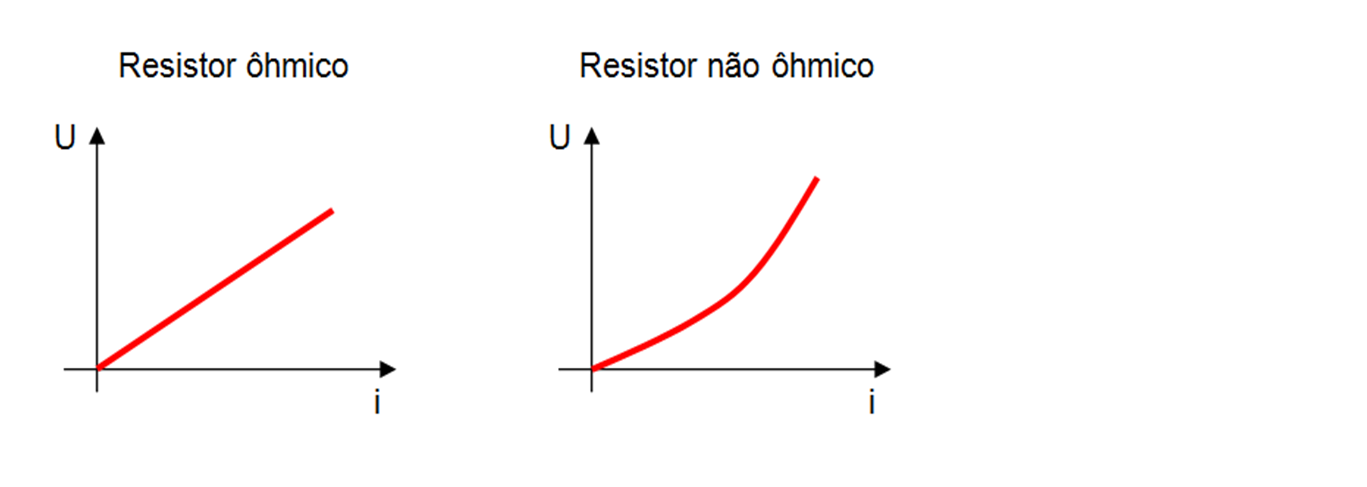
\includegraphics[width=0.9\linewidth]{Figuras/Ch12/ohmico.png}}
	\begin{block}{Diferença}
		\begin{itemize}
			\item \textbf{Ôhmico}: são lineares e $R$ é constante.
			\item \textbf{Não Ôhmico}: não são lineares e $R$ não é constante.
		\end{itemize}
	\end{block}

	\bigskip

	\begin{minipage}{0.49\linewidth}
		\centering
		\begin{tikzpicture}[scale=0.5]
			\draw (-4,-3) rectangle (4,3); %CLP
		\draw (-4,0) -- (-2.5,0); %Div in out
		\draw (-2.5,-3) -- (-2.5,3); %Div cartoes
		\draw (-1.5,-2.5) rectangle (0,2.5); %Mem dados
		\draw (0.5,-2.5) rectangle (3.5,-1); %Mem prog
		\draw (1,0) rectangle (3,2); %CPU
		\draw (-4,-5) rectangle (4,-3); %Alimentacao
		\draw (-2.5,4) rectangle (4,6); %Term de prog
		
		\draw (1,2.6) node {CLP};
		
		\draw (-3.25,1.5) node[text width=1.5cm,align=center,rotate=90] {\small Cartões de input};
		
		\draw (-3.25,-1.5) node[text width=1.5cm,align=center,rotate=90] {\small Cartões de output};
		
		\node at (2,1) {\small CPU};
		
		\node[rotate=90,text width=1.5cm,align=center] at (-0.75,0) {\small Memória de dados};
		
		\node[text width=2cm,align=center] at (2,-1.75) {\footnotesize Memória de programa};
		
		\node at (-6,0) {Campo};
		
		\node at (0,-4) {Alimentação};
		
		\node[text width=3cm,align=center] at (0.75,5) {Terminal de programação};
		
		\draw[-Latex] (-8,1.5) -- node[above] {Entradas} +(4,0);
		\draw[Latex-] (-8,-1.5) -- node[below] {Saídas} +(4,0);
		\draw[-Latex] (-2.5,1.5) -- +(1,0);
		\draw[Latex-] (-2.5,-1.5) -- +(1,0);
		\draw[-Latex] (0,1.5) -- +(1,0);
		\draw[Latex-] (0,0.5) -- +(1,0);
		\draw[Latex-] (2,0) -- +(0,-1);
		
		\draw[-Latex] (-1.5,4) -- +(0,-1);
		\draw[Latex-] (3,4) -- +(0,-1);
	\end{tikzpicture}
		
		Resistor ôhmico
	\end{minipage}
	\hfill
	\begin{minipage}{0.49\linewidth}
		\centering
		\newcommand{\innercolor}{gray!70!white}
	\newcommand{\outercolor}{gray!40!white}
	\newcommand{\leftcoil}{red!75!gray}
	\pgfmathsetmacro{\coilseparation}{0.02}
	
	\pgfmathsetmacro{\halflinewidth}{0.008}
	
	
	\begin{tikzpicture}[x={(\xx*1cm,\xy*1cm)},y={(\yx*1cm,\yy*1cm)},z={(\zx*1cm,\zy*1cm)}]
	\draw[\leftcoil, thick] (-0.02,5,1.125) -- +(0,2,0) (1.02,5,3.875) -- +(0,2,0);
	
	\draw[dashed,<->] ($ (-0.02,5,1.125)+(0,2,0) $) -- ($ (1.02,5,3.875)+(0,2,0) $);
	\node[rotate=85] at ($ (-0.02,5+2,1.125)!0.5!(1.02,5+2,3.875)+(0,0.2,0) $) {$ V_p $};
	
	\draw[-latex] (-0.02,6.5,1.325) -- node[above] {$ i_p $} +(0,-1,0);
	\draw[latex-] (1.02,0.02-0.5,1.3) -- node[above] {$ i_s $} +(0,-1,0);
	
	\filldraw[fill=\innercolor]  (0,1,1) -- (1,1,1) -- (1,4,1) -- (0,4,1) -- cycle;
	\filldraw[fill=\innercolor]  (1,4,1) -- (0,4,1) -- (0,4,4) -- (1,4,4) -- cycle;
	\filldraw[fill=\innercolor]  (0,0,0) -- (1,0,0) -- (1,0,5) -- (0,0,5) -- cycle;
	\filldraw[fill=\innercolor]  (0,0,5) -- (0,5,5) -- (1,5,5) -- (1,0,5) -- cycle;
	\filldraw[fill=\outercolor,even odd rule]    (0,0,0) -- (0,5,0) -- (0,5,5) -- (0,0,5) --cycle (0,1,1) -- (0,4,1) -- (0,4,4) -- (0,1,4) --cycle ;
	
	\begin{scope}
	\clip (0,3,1) -- (0,6,1) -- (0,6,4) -- (0,3,4);
	\foreach \z in {1.125,1.375,...,3.875}
	{   \draw[\leftcoil,thick] (0,5,\z) -- (-\coilseparation,5,\z) -- (-\coilseparation,4-\coilseparation,\z) -- (1+\coilseparation,4-\coilseparation,\z) -- (1+\coilseparation,4,\z);
	}
	\end{scope}
	
	
	\foreach \z in {1.25,1.75,...,3.75}
	{   \draw[blue,thick] (0,1,\z) -- (-\coilseparation,1,\z) -- (-\coilseparation,0-\coilseparation,\z) -- (1+\coilseparation,0-\coilseparation,\z) -- (1+\coilseparation,0,\z);
	}

	\draw[blue,thick] (1+\coilseparation,0+\coilseparation,1.1) -- +(0,-2,0) (-\coilseparation,1+\coilseparation,3.85) -- +(0,-3,0);
	
	\draw[dashed,<->] (1.02,-2+0.02,1.1) -- (-0.02,0.02-2,3.85);
	\node[rotate=-70] at ($ (1.02,-2+0.02,1.1)!0.5!(-0.02,0.02-2,3.85)+(0,-0.2,0) $) {$ V_s $};
	
	\draw[decorate,decoration={brace,amplitude=10pt},xshift=-4pt,yshift=0pt] (0,5,1.25) -- +(0,0,2.75);
	\draw[decorate,decoration={brace,amplitude=10pt},xshift=-4pt,yshift=0pt] (1.2,0,3.75) -- +(0,0,-2.6);
	\node[rotate=90] at (0,5.7,2.625) {$ N_p $ espiras};
	\node[rotate=-90] at (1.2,-0.5,2.5) {$ N_s $ espiras};
	
	\draw[dashed,postaction={decorate,decoration={markings,mark=between positions 0.1 and 1 step 0.2 with \arrow{Latex}}}] (0,4.5,0.5) -- (0,0.5,0.5) -- ++(0,0,4) -- ++(0,4,0) -- cycle;
	
	\draw[] (0,2.5,4.7)% -- +(0,-0.5,1.5)
	node[rotate=-10] {Fluxo magnético ($ \phi $)};
	
	\end{tikzpicture}
		
		Resistor não ôhmico
	\end{minipage}
}

\frame{
	\frametitle{Tipos de resistores}
	\centerline{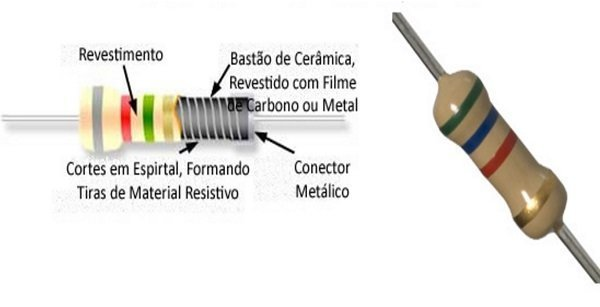
\includegraphics[width=0.9\linewidth]{Figuras/Ch12/carbono.jpg}}
	\begin{block}{Resistor de filme de carbono}
		\begin{itemize}
			\item Geralmente tem um corpo bege e são de baixa potência
		\end{itemize}
	\end{block}
}

\frame{
	\frametitle{Tipos de resistores}
	\centerline{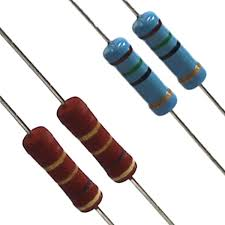
\includegraphics[width=0.4\linewidth]{Figuras/Ch12/metal.jpg}}
	\begin{block}{Resistor de filme de metal}
		\begin{itemize}
			\item Tipicamente de uma cor mais forte, como vermelho-tijolo ou verde-escuro, com especificações de potência mais altas.
		\end{itemize}
	\end{block}
}

\frame{
	\frametitle{Tipos de resistores}
	\centerline{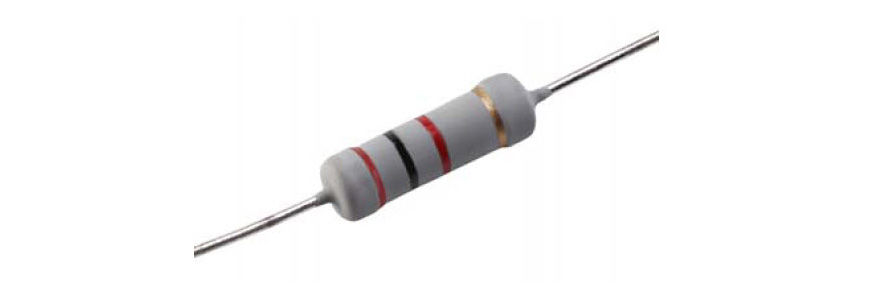
\includegraphics[width=0.9\linewidth]{Figuras/Ch12/oxido.jpg}}
	\begin{block}{Resistor de filme de óxido de metal}
		\begin{itemize}
			\item Normalmente tem uma cor pastel mais suave, e tem a especificação de potência mais alta ainda.
		\end{itemize}
	\end{block}
}

\frame{
	\frametitle{Código de cores}
	\centerline{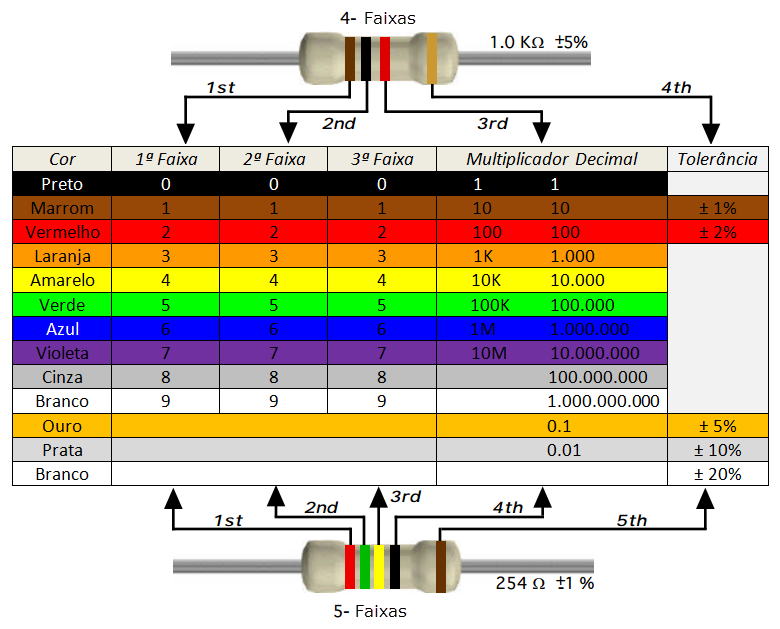
\includegraphics[width=0.82\linewidth]{Figuras/Ch12/tabela.png}}
}

\frame{
	\frametitle{Resistores variáveis}
	\centerline{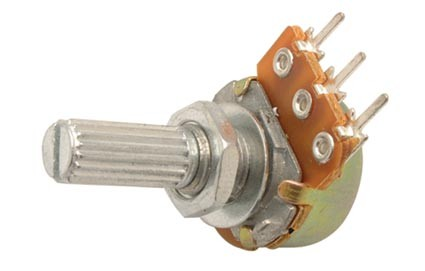
\includegraphics[width=0.5\linewidth]{Figuras/Ch12/potenciometro.jpg}}
	\begin{block}{Reostato x Potenciômetro}
		\begin{itemize}
			\item O \textbf{reostato} é um dispositivo de dois ou três terminais que é usado como resistor variável. Se ele for usado para controlar níveis de potência, então ele é normalmente denominado \textbf{potenciômetro}.
		\end{itemize}
	\end{block}
}

\frame{
	\frametitle{Aplicação de um potenciômetro}
	\centerline{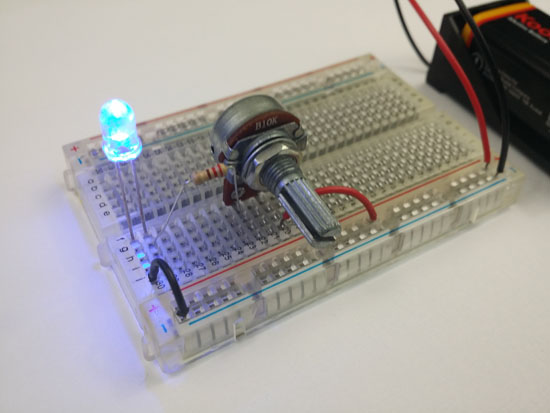
\includegraphics[width=0.8\linewidth]{Figuras/Ch12/potenciometro2.jpg}}
}

\frame{
	\frametitle{Termistores}
	\centerline{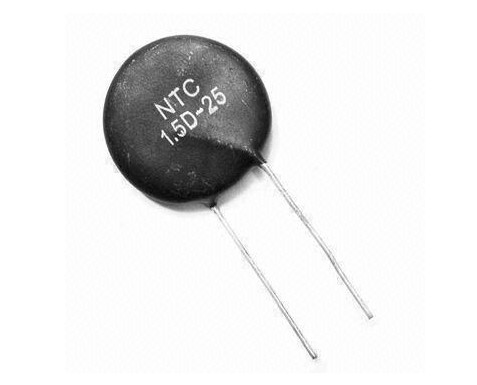
\includegraphics[width=0.5\linewidth]{Figuras/Ch12/termistores.jpg}}
	\begin{block}{Definição}
		\begin{itemize}
			\item São dispositivos elétricos que têm a sua resistência elétrica alterada termicamente, isto é, apresentam um valor de resistência elétrica para cada temperatura absoluta.
		\end{itemize}
	\end{block}
}

\frame{
	\frametitle{Termistores}
	\centerline{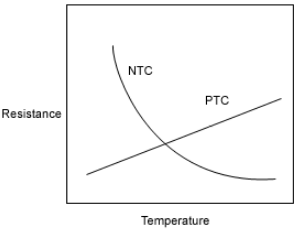
\includegraphics[width=0.5\linewidth]{Figuras/Ch12/ntc.PNG}}
	\begin{block}{Aplicação de um termistor}
		\begin{itemize}
			\item Controle de temperatura: termômetro digital. Podemos utilizar estes circuitos em automação de estufas, residencial/predial, controle de ar-condicionado, etc.
		\end{itemize}
	\end{block}
}

\frame{
	\frametitle{LDR}
	\centerline{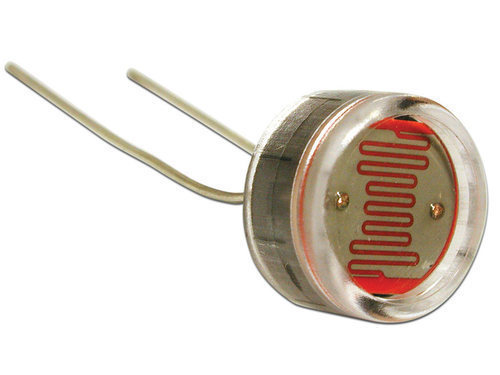
\includegraphics[width=0.5\linewidth]{Figuras/Ch12/LDR.jpg}}
	\begin{block}{Definição}
		\begin{itemize}
			\item Um LDR (Resistor Dependente da Luz) é um tipo especial de resistor que apresenta uma mudança em sua característica de resistência elétrica quando submetido à ação da luz.
		\end{itemize}
	\end{block}
}

\frame{
	\frametitle{LDR}
	\centerline{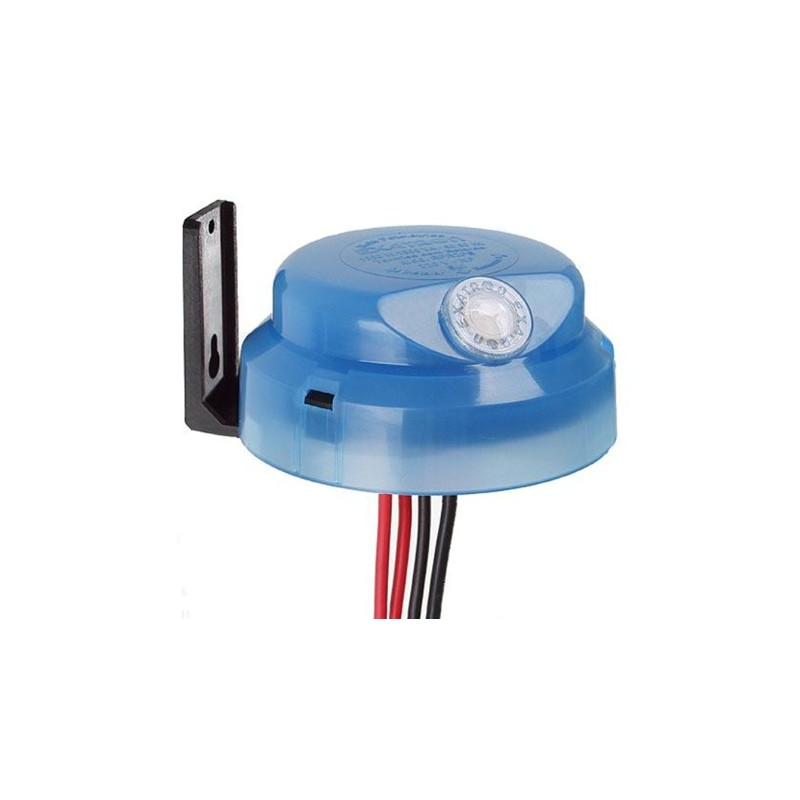
\includegraphics[width=0.5\linewidth]{Figuras/Ch12/fotocelula.jpg}}
	\begin{block}{Aplicação de um LDR}
		\begin{itemize}
			\item Controle automático de iluminação noturna
		\end{itemize}
	\end{block}
}

\subsection{}
\frame{
	\frametitle{Ohmímetro}
	\centerline{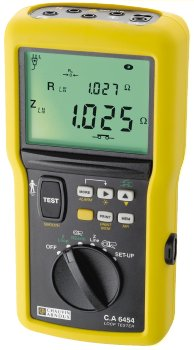
\includegraphics[width=0.25\linewidth]{Figuras/Ch12/ohmimetro.jpg}}
	\begin{block}{Atenção}
		Jamais conecte um ohmímetro a um circuito energizado!
	\end{block}
}

\section*{Exercícios}

\frame{
	\frametitle{Exercícios}
	\begin{block}{}
		01. Um resistor com os códigos de cores amarelo, violeta, marrom e prata que mede $\SI{492}{\ohm}$ está dentro da tolerância? Qual é o intervalo de variação da tolerância?

		\vspace{1cm}

		02. Se a resistência entre os terminais externos de um potenciômetro linear é de $\SI{10}{\kilo\ohm}$, qual a resistência entre o contato deslizante (móvel) e um dos terminais externos, se a resistência entre o contato deslizante e outro terminal externo é de $\SI{3.5}{\ohm}$?

	\end{block}
}

\section*{Referências}

\frame{
	\frametitle{Referências e Exercícios Complementares}
	\begin{itemize}
		\item Física, Ciência e Tecnologia – Vol 3. PENTEADO, Paulo César M; TORRES, Carlos Magno A. Ed. Moderna (2006)
	\end{itemize}
	%\centering{\alert{Página 36 - \textbf{1.6.1 até 1.6.5, 1.6.17 até 1.6.19}}} \\
	\centering{\alert{Lista de exercícios 12}}
}